% !TeX root = lsm.tex

\documentclass[sigconf]{acmart}
\usepackage[T1]{fontenc}
\usepackage[utf8]{inputenc} % Ensure proper character encoding
\usepackage{lmodern}
\graphicspath{{images/}{./}}  % first check 'images/' then the current directory


% % % % % % % % % % % % % % % % %
% Metadata – fill these in
% % % % % % % % % % % % % % % % %
\title{Heterogeneous computing in Log-Structured Merge Trees}
\author{Michael Almeida}
\affiliation{
  \institution{Harvard University}
  \city{Cambridge} \state{Massachusets} \country{USA}
}
\email{mia330@g.harvard.edu}

\acmISBN{05/15/25}
\acmDOI{0.0/XXXXXX.XXXXXXX}
\acmConference[CS-265 Spring 2025]{CS 265 - Big Data}
                {Cambridge}{MA}
\acmYear{2025}\acmMonth{05}
\begin{CCSXML}
<ccs2012>
 <concept>
  <concept_id>10010520.10010553.10010562</concept_id>
  <concept_desc>Computer systems organization~Parallel architectures</concept_desc>
  <concept_significance>500</concept_significance>
 </concept>
</ccs2012>
\end{CCSXML}
\ccsdesc[500]{Computer systems organization~Parallel architectures} % Add mandatory CCS concepts
% \ccsdesc[500]{Computer systems organization~Parallel architectures}
\keywords{Heterogeneous computing, LSM trees, GPU, FPGA, compaction, database systems} % Add mandatory ACM keywords
% \keywords{ACM \LaTeX\ template; sample document; your keywords}

% % % % % % % % % % % % % % % % %
% Packages
% % % % % % % % % % % % % % % % %
\usepackage{graphicx}   % for \includegraphics
\usepackage{booktabs}   % for \toprule, \midrule, \bottomrule in tables
\usepackage{subcaption} % sub-figures
\usepackage{amsmath}  % math
\usepackage{bookmark}
\usepackage{hyperref}    % clickable references
\hypersetup{%
  colorlinks=true,
  linkcolor=blue,
  citecolor=blue,
  urlcolor=blue
}


% % % % % % % % % % % % % % % % %
% Document begins
% % % % % % % % % % % % % % % % %
\begin{document}

\begin{abstract}
Log-Structured Merge Trees (LSM trees) are a popular data structure for
key-value stores, providing efficient write and read operations.
However, as the size of data and its complexity grows, the performance of LSM trees tends to degrade.
This is particularly true of the compaction process, which is typically a CPU-bottlenecked process.
To this end, we review the state-of-the-art in heterogeneous computing for LSM trees, focusing on GPU and FPGA-based approaches.
We analyze the performance and architectural trade-offs of these approaches, including their parallelism models, memory and communication strategies, reconfigurability, and energy efficiency.
We also identify gaps in the current research and propose future directions for improving the performance of LSM trees using heterogeneous computing.
We conclude that while GPU and FPGA-based approaches show promise, with CUDA streams being of expectional potential, there is still much work to be done in terms of optimizing performance, reconfigurability, and energy efficiency.
\end{abstract}
\settopmatter{printacmref=true} % Enable ACM reference format
\settopmatter{printacmref=false}
\maketitle

\section{Introduction}
  \subsection{Motivation}
   Key-Value stores and, subsequently, LSM trees have become a very popular data structure for real world, write heavy workloads. These include NoSQL databases, such as LevelDB and RocksDB, which are widely used in industry.
    Moreover, since the advent of the Cloud and cheaper SSDs, LSM trees have become even more relevant as they are able to efficiently handle large amounts of data.
    Due to the LSM tree's design, it's both able to soak up an extremely high write throughput, while also being able to provide amoritized read performance for more recent data.
    A particularly elucidating case study for this is the work done by \cite{rocksdb}, which shows that RocksDB 4.5M-7M read QPS for point lookups with sustained writes. 4M-6M QPS prefix range scans with sustained writes.
    In scenarios such as E-commerce, social media, and IoT applications, the ability to handle large amounts of data efficiently is crucial. Moreover, we see that real workloads tend to retrieve more recent data more often.

    KV-Stores build on the LSM tree design typically tend to have other features, such as Bloom filters and fence pointers, which help to reduce the number of I/O operations needed to retrieve data, and research has been done to further optimize these sub structures.\cite{dayan2017monkey}
    Despite all the effort spend on hardware software co-design for CPU based LSM trees, as the size of data and its complexity grows, the performance still tends to degrade. This is particularly true of the compaction process, which is typically a CPU-bottlenecked process.
    Research has also been done to optimize the compaction process, such as \cite{dayan2018dostoevsky} \cite{dayan2019log} which aim to improve the compaction policies associated with LSM trees. However, these optimizations are limited by the CPU's performance and the memory bandwidth of the system.

    That being said, desipite the enormous success of LSM trees, and the massive amount of value that has been delivered, we continue to seek ways to improve these systems and make them more efficient. To this end, we review the state-of-the-art in heterogeneous computing for LSM trees, focusing on GPU and FPGA-based approaches. We analyze the performance and architectural trade-offs of these approaches, including their parallelism models, memory and communication strategies, reconfigurability, and energy efficiency.

  \subsection{Rise of Heterogeneous Hardware}

  \subsubsection{Graphics Processing Units (GPUs)}
  Modern GPUs provide massive data-parallel compute resources and very high memory bandwidth, making them attractive targets for offloading the most compute-intensive phases of LSM-tree compaction.
  Their single-instruction, multiple-thread (SIMT) execution model can launch thousands of lightweight threads in parallel—each executing the same instruction on different data—perfectly matching the parallel merge and sort kernels that underpin compaction.

  The GPU memory hierarchy further amplifies this advantage.  At the top sits global memory: the largest but slowest on-device storage, which holds the bulk of SSTable data.
  Beneath that, shared memory provides a small, low-latency scratchpad for intra thread-block communication, and registers offer per-thread storage at the highest speed.
  GPUs also expose constant memory (read-only and cached) and texture memory (optimized for 2D spatial locality), though compaction kernels typically focus on tiling data between global, shared, and register spaces to minimize global-memory traffic.

  In recent years, frameworks such as CUDA and OpenCL have made these hardware features accessible via high-level APIs.
  This democratization of GPU programming has driven widespread adoption in data-processing fields—from machine learning to scientific computing and, increasingly, database systems.
  NVIDIA's latest architectures (e.g.\ Hopper and Blackwell) have continued to push peak memory bandwidth and reduce latency, directly benefiting workloads like LSM compaction that are sensitive to both.

  Early GPU-LSM work by Ashkiani et al.\ demonstrates that a dynamic GPU-resident dictionary with batch-merge compactions on the device can sustain up to 225 M inserts/sec, and deliver 75 M/32 M/23 M QPS for lookup, count, and range operations under sustained writes \cite{ashkiani2018gpu}.  This work specifically builds a LSM backed Key-Value storage on the GPU Memory-- and does not deal with compactions; but serves to highlight the naturally paralellizable workload of typical LSM workloads.
  Building on this, Zhou et al.\ show that integrating CUDA streams with GPUDirect Storage—thereby overlapping I/O transfers and compaction kernels—yields 2-3x end-to-end throughput improvements compared to CPU-only designs \cite{zhou2024gpuaccel}.

  \subsubsection{Field-Programmable Gate Arrays (FPGAs)}
  FPGA;s are a reconfigurable class of hardware devices composed of lookup tables (LUTs), flip-flops, on chip DRAM, and other hardware elements-- and have the added advantage that they can scale with the amount of resources they provision and not due to any software.
  Practically, this means that FPGAs tend to ship without an operating system, and instead rely on a hardware description language (HDL) to describe the hardware that is to be implemented. Software Engineers can then use high-level synthesis (HLS) tools to compile C/C++ like code into a HDL, which is then synthesized into a bitstream that can be loaded onto the FPGA. This allows for a high degree of flexibility and reconfigurability, as the hardware can be changed on-the-fly to adapt to different workloads.
  FPGAs tend to be deployed in situations where the algorithmic workload is highly sequential, and the data is highly structured. This is because the hardware units can be highly optimized to specific workloads, and the data can be streamed through the hardware in a highly efficient manner.

  In a typical FPGA-accelerated LSM tree workflow, SSTable data streams from SSDs over PCIe into on-card buffers implemented in on-chip RAM.
  Custom comparators and merge networks—crafted in HDL or then execute streaming compactions in deeply pipelined stages.
  Each cycle, data flows through comparator trees, prefix compressors, and write schedulers without any control-flow overhead, achieving sustained throughput far beyond what CPUs can deliver for the same workload. \cite{zhang2020fpga}

  \begin{itemize}
    \item \em Deterministic pipelines: Fixed-latency stages ensure predictable performance.
    \item \em Fine-grained \em parallelism: Multiple merge units can operate in parallel on independent data streams.
    \item \em On-chip buffering: S/BRAM holds hot key ranges and intermediate results, reducing off-chip memory traffic.
  \end{itemize}

  In the cloud, FPGAs are deployed in a variety of configurations, and the reader is encouraged to refer to the work done by \cite{bobda2022future} for a in depth survey of successful, massively deployed FPGA systems in use at Tencent and Microsoft.
  Notably, the most interesting deployment strategies-- atleast with respect to accelerating LSM trees and that we see used in this survey, are the following:
   \begin{itemize}
    \item Bump-in-the-Wire: FPGA sits between CPU and storage (or network), filtering and merging data on the fly.  Microsofts Catapult v2 uses this model for network packet processing and search index merging in Azure datacenters. \cite{bobda2022future}
    \item Co-Processor: FPGA is PCIe-attached or Ethenret attached to a host node, offloading compute-intensive tasks while the CPU handles control and metadata.  Alibaba Cloud’s F3 and AWS F1 instances follow this pattern, allowing customers to accelerate databases, genomics, and AI inference. \cite{bobda2022future}
    \item Smart SSD / Computational Storage: Emerging SSDs integrate FPGA logic alongside NAND controllers, enabling compaction to occur inside the storage device itself (e.g.\ Samsung SmartSSD).
  \end{itemize}
\begin{figure}[ht]
  \centering
  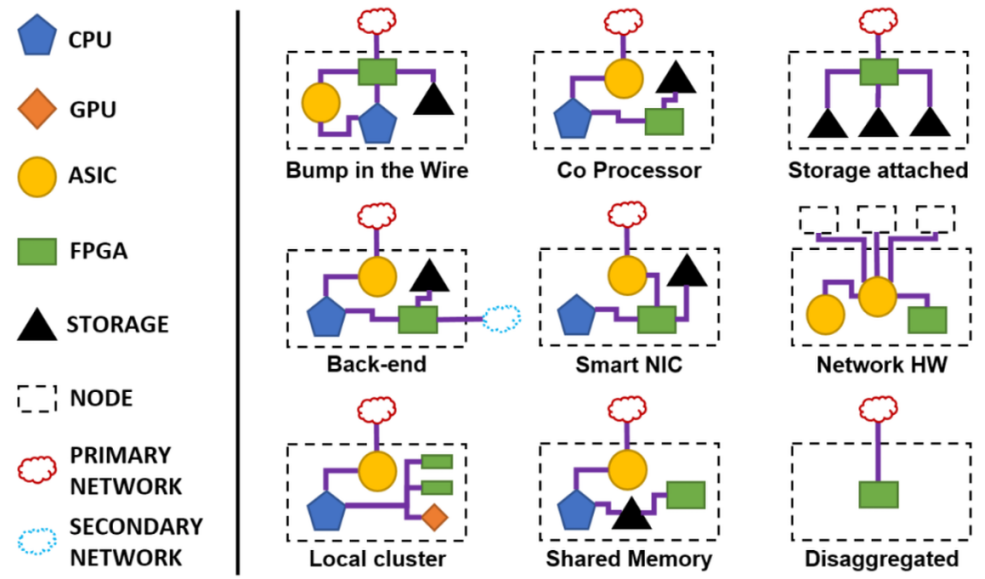
\includegraphics[width=0.5\textwidth]{bobka.png}
  \caption{Different architectures from Bobda et al\cite{bobda2022future}. This figure illustrates FPGA deployment strategies.}\label{fig:SSTable} % Add description for accessibility
  \begin{description}
    \item[Bump-in-the-Wire] FPGA sits between CPU and storage (or network), filtering and merging data on the fly.  Zhang et al uses this design for their FPGA compaction accelerator design.
  \end{description}
\end{figure}


  By integrating an FPGA accelerator into the LSM pipeline, the host CPU is freed from merge stages and can focus on memtable management and query dispatch, leading to higher overall throughput and lower tail latencies in write-heavy environments.


  \subsection{Research Questions and Angle}
  This survey is structured around the following research questions:

    \begin{itemize}
      \item \textbf{RQ1:} Is it truly viable to offload LSM-Tree computations (compaction and otherwise) to GPUs and FPGAs? What performance and cost improvements to these accelerated paradigms produce compared to the very battletested CPU-only paradigms.
      \item \textbf{RQ2: } What are the key architectural tradeoffs between GPU-Based (SIMT, High Bandwidth memory) and FPGA-based (Dataflow pipelines, low latency mem access) LSM Accelerators in terms of throughput and tail latency?
      \item \textbf{RQ3:} What are the key differences in programming models and reconfigurability between GPU and FPGA-based LSM accelerators? How do these differences impact the design of LSM Trees and, by extension, to what extend can LSM-trees be disaggregated from the CPU host?:w
      \item \textbf{RQ4:} What are the key gaps in the current research on heterogeneous computing for LSM trees? What are the most promising future directions for improving the performance and efficiency of LSM trees using heterogeneous computing?
    \end{itemize}

    We adopt a quantitatively driven, systems-level perspective, rigorously comparing published performance, energy, and cost metrics to move beyond vendor claims. Our goal is to uncover the true delta achievable with heterogeneous LSM-tree designs and to draw generalizable lessons for disaggregated storage and near-data processing architectures.


\section{Background}

  \subsection{LSM-Tree}
    Log-Structured Merge Trees (LSM trees) are a popular data structure for key-value stores, providing efficient write and read operations.
    A LSM Tree typically comprises of different datastructures working together in unison.

      \begin{figure}[htbp]
      \centering
      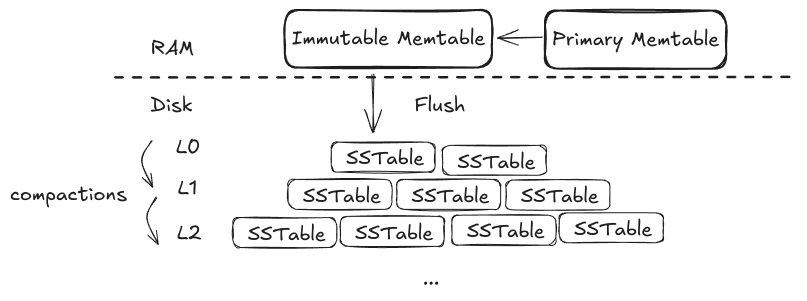
\includegraphics[width=0.4\textwidth]{sstable.png}
      \caption{LSM Tree Architecture}\label{fig:LSM}
      \begin{description}
        \item[Memtable] In-memory data structure for fast writes.
        \item[SSTable] Sorted, immutable data structure for efficient reads.
        \item[Compaction] Merging and purging of SSTables to maintain performance.
      \end{description}
      \end{figure}

      \subsection{Memtable and the Write Path}
      A \emph{memtable} is the in-memory write buffer holding the most recent updates.  It is usually implemented as a concurrent skiplist (though red–black trees or even growable vectors are also used) to provide low-latency inserts and lookups.  Once the memtable reaches its size threshold, it is \emph{flushed}—sorted and serialized—into an on-disk Sorted String Table (SSTable).

      To enable asynchronous flushing, systems maintain two memtables in tandem.  When the active memtable fills up, a fresh one is allocated and becomes the new write target, while the old memtable is marked \emph{immutable}.  An immutable memtable still services reads (so in-flight queries can see the latest data) but no longer accepts writes; once its flush to disk completes, it is discarded.

      \subsection{SSTable and the Read Path}
      An SSTable is an immutable, sorted file of key-value entries on disk.  Lookups proceed in two stages:
      \begin{enumerate}
        \item Check the memtable (and any immutable memtable).
        \item If not found, probe each level's SSTables, newest first.
      \end{enumerate}
      To avoid scanning every SSTable or every block within one, modern engines layer on:

      \paragraph{Bloom Filters}
      A compact, probabilistic bit-array structure that quickly tests “definitely not present” versus “possibly present.”  If the filter says “absent,” the SSTable can be skipped altogether.

      \paragraph{Fence Pointers}
      A small index—e.g.\ one pointer per 4 KB block—that maps key ranges to file offsets.  On a positive Bloom filter hit, fence pointers let you jump directly to the block containing the key, avoiding a full scan or binary search of the SSTable.

      Above these, further optimizations—prefix encoding, per-block compression, and optimized on-disk layouts—reduce I/O volume and improve read performance.

      \subsection{LSM Tree Point Query}
        \label{sec:readpath}

      \begin{figure*}[h]
        \centering
        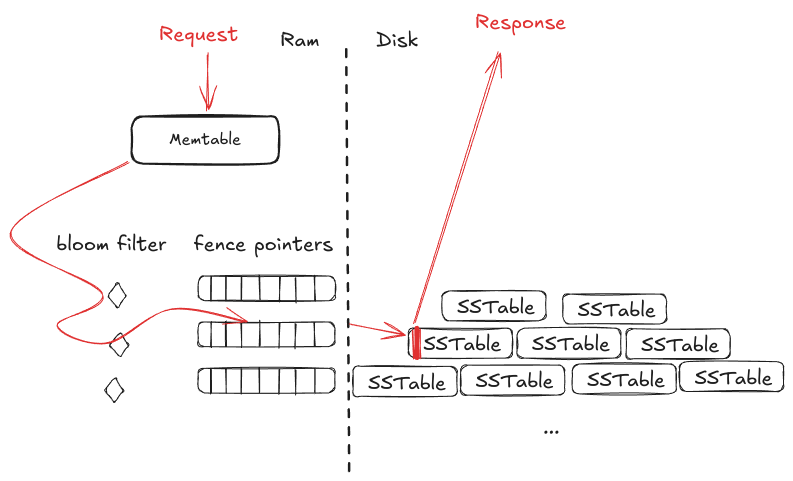
\includegraphics[width=0.5\textwidth,height=0.3\textheight]{read path.png}
        \caption{Point lookup flow in an LSM tree: memtable, Bloom filters, fence pointers, then SSTable block fetch.}
        \label{fig:readpath}
      \end{figure*}

      A point lookup in an LSM tree proceeds as follows:

      \begin{enumerate}
        \item \textbf{Memtable check (in RAM).}
          Query the active memtable (and any immutable memtable being flushed).
          If the key is found, return its value immediately.
        \item \textbf{Bloom filter probe (in RAM).}
          For each candidate SSTable (newest level first), check its in‐memory Bloom filter.
          A “no” answer means the SSTable is skipped; a “yes” means “possibly present.”
        \item \textbf{Fence pointer lookup (in RAM).}
          For each SSTable whose Bloom filter returned “yes,” consult its fence‐pointer array
          to identify the precise block offset containing the key.
        \item \textbf{SSTable block fetch (from disk).}
          Issue a single block read (e.g.\ 4 KB) at the offset given by the fence pointer.
        \item \textbf{In-block search and return.}
          Scan or binary-search within the fetched block to locate the key/value pair, then return it.
      \end{enumerate}

      \paragraph{Caveats and Refinements}
      \begin{itemize}
        \item \textbf{Bloom-filter false positives.}
          A “yes” from the filter can be wrong, costing an extra block read even if the key is absent.
        \item \textbf{Level hierarchy.}
          SSTables are organized in levels (L0, L1, …), and lookups scan levels in newest‐first order.
        \item \textbf{In-memory caches.}
          Systems often cache hot blocks or pages, letting some lookups bypass disk entirely.
        \item \textbf{Range scans.}
          For range queries, multiple SSTables may contribute results; engines merge‐scan blocks in key order across levels.
      \end{itemize}

    \section{Compaction}
      \label{sec:compaction}

      Compaction is the background merge process that transforms multiple on–disk SSTables into larger, coalesced SSTables, reclaiming space from deleted or overwritten keys and bounding the number of files that must be consulted on reads.  While memtable flushes keep write latency low, compaction ensures long–term storage efficiency and read performance at the cost of CPU and I/O resources.

      \subsection{Compaction Strategies}
      Two primary compaction styles are used in practice:

      \begin{figure}
        \centering
        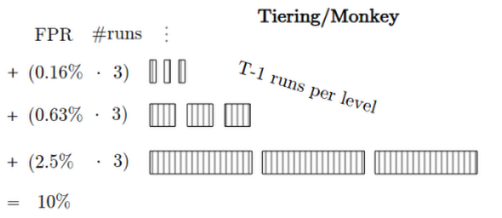
\includegraphics[width=0.5\textwidth]{compaction_lsm.png}
        \caption{tiered compaction strategies from Dayan et al \cite{dayan2019log}}
        \label{fig:compaction_zhou:ways}
      \end{figure}

      \begin{description}
        \item[Leveled Compaction]
          Each level \(L_i\) is size‐bounded (e.g.\ \(10\times\) the size of \(L_{i-1}\)).  When level \(L_{i-1}\) grows too large, SSTables are merged into \(L_i\).  This minimizes read amplification—at most one SSTable per level—but increases write amplification due to repeated merges.
        \item[Tiered Compaction]
          SSTables in each level accumulate into \emph{tiers} (batches) of \(k\) files before merging them all at once into the next level.  This reduces write amplification by merging fewer times, but increases read amplification since multiple SSTables per level must be consulted on point reads.
      \end{description}

      The compaction ratio is defined as the ratio of the size of SSTables in level \(L_i\) to the size of SSTables in level \(L_{i-1}\).  For example, if level \(L_0\) has 10 GB of data and level \(L_1\) has 100 GB of data, the compaction ratio is 10.  A higher compaction ratio means that more data is being compacted at once, which can lead to better performance but also higher write amplification.
      When the compaction ratio is equal to 2, the leveled compaction strategy is equivalent to the tiered compaction strategy. This is because the leveled compaction strategy will merge two SSTables into one, while the tiered compaction strategy will merge two tiers of SSTables into one.

      Likewise, then the compaction ratio is equal to 1, basically this deteriorates into just a simple merge sort, where every sstable is merged into one. On the other asymptotic end, if the compaction ratio is equal to infinity, it's essentially just having one Key Value pair in each sstable, and it degrades to just having a vector.

      \subsection{Compaction Workflow and Triggers}
      \begin{enumerate}
        \item \textbf{Memtable Flush:}  When the active memtable fills, it is flushed to a new SSTable in level 0.
        \item \textbf{Size/Count Thresholds:}
          \begin{itemize}
            \item For leveled compaction, each level has a maximum total size.
            \item For tiered compaction, each level has a maximum SSTable count.
          \end{itemize}
        \item \textbf{Background Merge:} A background thread (or pool) selects candidate SSTables, reads and merges their sorted runs while removing tombstones, and writes out new SSTables in the next level.
        \item \textbf{Concurrency Control:} Modern engines parallelize compactions across levels or key ranges, but excessive concurrency may exacerbate write amplification or contend for disk bandwidth.
      \end{enumerate}

      \subsection{Cost Model}
      Compaction incurs three forms of overhead:
      \begin{itemize}
        \item \textbf{Write Amplification}
          Additional bytes written due to repeated merging of the same key across levels.
        \item \textbf{Read Amplification}
          Number of SSTables read per lookup; minimized by leveled compaction.
        \item \textbf{Space Amplification}
          Temporary extra storage used while old and new SSTables coexist.
      \end{itemize}
      Tuning compaction parameters (memtable size, level fan-out, concurrency) balances these trade-offs for a given workload.

      \subsection{Software Optimizations and Limits}
      The following papers that were studied in class propose software optimizations to the compaction process through better policies and hardware/software co-design:
      \begin{itemize}
        \item \emph{Dostoevsky} \cite{dayan2018dostoevsky} removes unnecessary merges by adaptively skipping SSTables.
        \item \emph{LSM‐bush / Wacky} \cite{dayan2019log} reorganizes levels into a continuum to smooth write peaks.
      \end{itemize}
      However, compaction remains largely CPU-bound: sorting and merging large runs stress cores and memory bandwidth long before SSD I/O is saturated because of heavy data movement-- especially for write-heavy workloads.  This is where heterogeneous hardware can help.

      \subsection{Motivation for Hardware Offload}
      Compaction is a well studied problem in LSM Design and it is known to consume a dominating amount of system resources-- especially on write heavy workloads.
      Because compaction kernels consist of parallel sort/merge and probabilistic filter probes, they map naturally to heterogeneous devices:
      \begin{itemize}
        \item \textbf{GPUs:} Thousands of SIMD lanes can run merge kernels in parallel and overlap I/O via CUDA streams \cite{ashkiani2018gpu, zhou2024gpuaccel}.
        \item \textbf{FPGAs:} Custom, deeply-pipelined merge networks and on‐chip buffers eliminate CPU‐side overhead and deliver predictable low‐latency compactions \cite{quraishi2025saf,zhang2020fpga}.
      \end{itemize}
      In the next sections, we explore these GPU and FPGA accelerated compaction designs in detail.

      \subsection{GPU Basics}
        GPUs expose thousands of parallel compute units organized in a Streaming Multiprocessors-- also called CUDA Cores. These SMs execute in a single-instruction, multiple-thread (SIMT) model.  In GPUs (NVIDIA), the hardware hierarchy consists of:
        \begin{itemize}
          \item \textbf{Registers}: private to each thread, the fastest storage.
          \item \textbf{Shared memory}: a small, programmer managed bank shared by all threads in a block.
          \item \textbf{L1/L2 caches}: hardware managed caches where each SM has its own L1, and all SMs share an L2.
          \item \textbf{Global (DRAM) memory}: the largest, highest latency pool accessible by all threads. Typically the CPU Loads data into here such that the GPU can access it.
        \end{itemize}
        Because global DRAM bandwidth is often the bottleneck, kernels must be written to coalesce memory accesses so that consecutive threads touch consecutive addresses in global memory \cite{ashkiani2018gpu}. This basically means positioning computation such that elements are accessed sequentially, from shared memory.

        NVIDIAs CUDA programming model lets developers write a Cstyle kernel for a single thread; the runtime then schedules many such threads in blocks of up to 1\,024 threads per SM, organized into “warps” of 32 threads each, which execute in lockstep \cite{ashkiani2018gpu}.  This make GPUs ideal for data-parallel operations such as bulk sorting, merging, and hash-based probing \cite{ashkiani2018gpu, zhou2024gpuaccel}.

        At a higher level, common GPU resident data structures include:
        \begin{itemize}
          \item \emph{Unordered arrays} for simple bulk storage.
          \item \emph{Sorted arrays} for fast binary-search queries.
          \item \emph{Hash tables} for constant-time lookup of individual keys.
        \end{itemize}
        However, mutable dynamic structures supporting both updates and range queries have historically required rebuilding on the CPU; only recently have efforts such as GPU LSM enabled fully dynamic ordered dictionaries on GPU \cite{ashkiani2018gpu}.

        \subsection{NVIDIA GPUDirect Storage}
        NVIDIA GPUDirect Storage (GDS) enables direct DMA transfers between GPU device memory and NVMe SSDs, bypassing host DRAM and CPU involvement \cite{zhou2024gpuaccel}.  Without GDS, an SSTable read would flow:
        \[
          \text{SSD} \;\xrightarrow{\text{DMA}}\;\text{Cpu DRAM}
          \;\xrightarrow{\text{PCIe}}\;\text{GPU DRAM}
        \]
        with two explicit copies.  GDS collapses this into:
        \[
          \text{SSD} \;\xrightarrow{\text{DMA}}\;\text{GPU DRAM}
        \]
        eliminating the intermediate transfer and CPU overhead.  In LSM tree compaction—where large sorted runs must be ingested and emitted in bulk—GDS can increase end-to-end throughput and free CPU cycles for other tasks \cite{zhou2024gpuaccel}.

      \subsection{FPGA Basics}
        Field-Programmable Gate Arrays (FPGAs) are reconfigurable hardware fabrics composed of three primary resource types:
        \begin{itemize}
          \item \textbf{Logic elements}: Configurable Look Up Tables (LUTs) and registers that implement arbitrary combinational and sequential logic.
          \item \textbf{Block RAM (BRAM) and DSPs}: On chip SRAM blocks provide lowlatency storage, while dedicated Digital Signal Processors (DSP) slice accelerate arithmetic without consuming general logic units.
          \item \textbf{Programmable interconnect and I/O interfaces}: A grid of reprogrammable wiring links all resources, and FPGAs attach to the host (e.g., via PCIe or Ethernet) for fast data movement.
        \end{itemize}
        Programmers target FPGAs by writing hardware descriptions (e.g., in Verilog/VHDL) that map custom, deeply pipelined circuits onto these resources. Unlike CPUs or GPUs, which schedule instructions at runtime, an FPGAs entire computation is laid out in hardware: data flows through user-defined pipelines and buffers with no implicit controller.

        This spatial, dataflow execution model is ideal for merge heavy workloads such as LSM-tree compaction. By instantiating multiple parallel comparator trees and using BRAM as streaming FIFOs, an FPGA can merge sorted runs in hardware at the full memory line rate—reading, comparing, and writing continuously—thereby offloading and accelerating the merge-sort stages far beyond what a software implementation on a CPU can achieve. \cite{Dann24}


       \section{GPU-Based Approaches}

        \subsection{GPU LSM (Ashkiani et al.)}
        In GPU LSM, Ashkiana et al. developed a dynamic dictionary data structure based off of the LSM tree. This paper does not deal with accelerating compaction specifically, but rather with the design of batch operations that are consistent with the GPUs bulk programming model. Practicaly, this means that queries do not modify the structure and thus can all be run in parallel. However, updates pose a challenge with regards to correctness \cite{ashkiani2018gpu}.
        
        \begin{itemize}
          \item \textbf{Dynamic dictionary on GPU:}
            GPU LSM is the first fully mutable dictionary data structure implemented entirely in GPU memory.
            It maintains a multi-level, LSM-tree-style layout of sorted arrays (levels) in DRAM on the GPU, enabling insertions, deletions, and queries without round trips to the CPU or disk \cite{ashkiani2018gpu}.
          \item \textbf{Merge based batch inserts and tombstones:}
            Updates are applied in batches of size $b$. Each batch is sorted on the GPU and then merged up through successive levels (of size $b2^i$) in a binary counter fashion.
            Deletions are handled via tombstone records inserted like any other update; stale entries are purged later during a periodic cleanup pass \cite{ashkiani2018gpu}.
          \item \textbf{Query kernels:}
            Point lookups launch parallel binary searches across all occupied levels, returning the most recent (lowest lvl) match and filtering out tombstones.
            Range and count queries gather per-level subranges in parallel, concatenate them, and then compact out duplicates and tombstones in a post processing kernel \cite{ashkiani2018gpu}.
          \item \textbf{Performance vs.\ sorted array:}
            On an NVIDIA K40c, GPU LSM attains up to 225 M updates/sec—over 13x faster than a GPU-resident sorted-array merge baseline—while still supporting 75 M lookups/sec, 32 M count queries/sec, and 23 M range queries/sec.
            The trade‐off is that queries run about 2x slower than a monolithic sorted array, in exchange for dramatically higher update throughput \cite{ashkiani2018gpu}.
        \end{itemize}

        \subsection{LevelDB + GPU Compaction (Zhou et al.)}
        Zhou et al. introduce a hierarchical apporach to GPU-Accelerated compaction. Under the observation that The early levels in LevelDB based LSM trees are typically small, they make a distinction and propose two novel compaction methods that build on the work of previous researchers. 
        Moreover, they propose a new execution style that levereges recent advances in GPU hardware to bridge the memory shuttling gaps that are present in any GPU based acceleration apporach.
        
        \begin{itemize}
          \item \textbf{Q-Compaction (upper levels) vs.\ C-Compaction (lower levels):}
            \emph{Q-Compaction} offloads entire compaction of small, top-of-tree SSTables (L0→L1, L1→L2) to the GPU, running parse-sort-write fully on CUDA.
            \emph{C-Compaction} handles large, lower-level merges by having the GPU parse and sort key-value pairs, then the CPU performs garbage-collection of tombstones, and finally the GPU serializes filtered data into new SSTables \cite{zhou2024gpuaccel}.
          \item \textbf{CUDA streams and GPUDirect Storage:}
            Asynchronous CUDA streams overlap data transfer and compute, streaming chunks of SSTables into GPU memory while prior batches are being sorted or written in a pipelined fashion.
            NVIDIA GPUDirect Storage enables direct SSD→GPU DMA for SSTable I/O, bypassing host DRAM and CPU copies. \cite{zhou2024gpuaccel}.
          \item \textbf{Throughput and mixed workload gains:}
            Compared to vanilla LevelDB compaction, the GPU accelerated approach achieves up to 3.6x higher compaction throughput.
            Measured end-to-end, write throughput improves by up to 2.34x, and mixed read/write throughput by up to 2.02x; in all cases outperforming an earlier GPU-offload prototype (LUDA) by over 1.5x \cite{zhou2024gpuaccel}.
        \end{itemize}

\section{FPGA-Based Approaches}
  \subsection{SAF (Quraishi et al.)}
  Quraishi et al. introduce the Scalable Acceleration Framework (SAF), which targets the inflexibility of existing FPGA clusters with regards to scaling. These existing fpga clusters provide great throughput and low latency, but rely on 
  HOST-FPGA and fpga-interlinks to communicate with eachother. Practically, this introduces difficulty in disaggregated scaling-- i.e. being able to add FPGAs on the fly typcially isn't time nor cost effective. 
  They content that this inflexibiltiy limits FPGA adoption in the cloud, and propose a framework that allows for efficient inter-FPGA communication, as well as a self-discovering protocol.:w 
    \begin{itemize}
      \item \textbf{Ethernet shell and hot-plug discovery}
          In order for FPGAs to function as standalone network nodes, the authors developed a custom shell-- a \emph{SAF Shell}, that implements networking and self-update protocols. This is in contrast to traditional PCIe, and instead a standard network 
          connects 20 FPGAs with a commodity 10GbE switch. This Shell routes packages between FPGAs and the host, and supports several accelerator protocols to fasciliate discovery, reconfiguration, remote configuration, and remote dispatch \cite{quraishi2025saf}.
      \item \textbf{Parallel partial reconfiguration}
          The SAF shell supports partial reconfiguration, allowing for the dynamic loading of new bitstreams into the FPGA fabric. This allows for the dynamic loading of new accelerators, and the ability to switch between different workloads on the fly \cite{quraishi2025saf}.
      \item \textbf{Compaction Protocolos}
          The SAF paper is a general framework to accelerate any workload, and the authors don't implement an explicit compaction protocol. However, in principle, the SAF Shell would allow LSM-tree compaction kernels (and other data intensive tasks) to dynamically scale on any FPGA fabric. 
          This is important because there is a stated gap in existing research, whereby FPGAs are forced to co-locate with the CPU and are otherwise not able to scale independently-- which inherently limits the ability to create a disaggregated design space. 
      \item \textbf{Performance Gains and tradeoffs}
          The SAF framework demonstrated substantion improvements in deployment flexibility and reconfiguration speed, with purpoted experiments showing 2x-13x faster reconfiguration times compared to traditional PCIe-based systems.
          Morever, FPGAs mid execution yielded up to 25\% reduction in application runtime and energy costs-- as the workload is simply able to complete more quickly, and the extra FPGAs can then be removed / shut off. SAF prioritizes scalability and modularity instead of direct latency as they sacrificed FPGA interlink for Ethernet connection.
    \end{itemize}

  \subsection{On-Card Compaction Modules (Peng et al.)}
  Peng et al. propose hardware-software codesigned compaction system where the FPGA communicates directly with the storage medium and performs compaction on chip. They also discuss prior research that has been explored on FPGAs embedded with CPUs-- and build a full hardware test platform that thusly assesses the high computation costs and read/write/space amplification of compactions on a systematic level.
  In this, an architecture is proposed whereby a custom compaction module and flash controller is implemented on a Xilinix fPGA, alongside an embedded softcore MicroBlaze cpu that performs the control logic amd coordinates operations.

    \begin{itemize}
      \item \textbf{Compaction Module}
        The Compaction module is the heart of the design-- it merges two sorted streams of key-value pairs. It includes sub-modules for reading data from FIFOs, key comparators, merging, and writing results. According to the paper, the 
        comparator and merger submodules accept keys from two input FIFOs and use dictionary-order comparision to output the merged sequence in sorted order. After sorting and merging, the Encoder module uses prefix compression to store the sorted keys-- and outputs fixed-wdith 
        32 bit data-- specifically in a compact format conforming to its SSTable block format. 
      \item \textbf{NAND Module}
        A three-layer controller (command decoder, timing FSM, PHY interface) issues reads/writes directly to on-card flash chips via AXI-DMA, eliminating host I/O and letting the compaction engine operate \emph{in situ} on raw SSTable pages.
      \item \textbf{MicroBlaze CPU}
        This is where the co-design aspect lies in that the MicroBlaze CPU refers to a soft-core SPU. The main host running the LSM-tree can offload all of the compaction logic to the MicroBlaze cpu, and this cpu will coordinate everything the compaction job needs as far as the FPGA is concerned.
      \item \textbf{Performance Gains and tradeoffs}
        Offloading LevelDB's compaction process to the FPGAs is reported to show \emph{significant} speedups-- in tests, up to 11\% faster compaction that just software compaction. Specifically, with 8192 KeyValue entries to merge, the FPGA completed the task 11x faster than the LEvelDB baseline. 
        This comes from both the higher raw processing speed, and further elimination of most of the data transfer overhead. 
    \end{itemize}

    Overall, the architecture is a self-contained compaction accelerator: the CPU host device triggers a compaction job and the FPGA cards do all the work from reading the tables off disk and writing them back to disk; alleviating all of the IO overhead from the Host. Specifically, this IO overhead comes from processes such as the Operating System.
    Notably, there could be a lot of security issues when reading and writing just using the block storage device-- and the Operating system provides a lot of this security. 


  \subsection{FPGA Co-Processor in DB Server (Zhang et al.)}
  Zhang et al.~\cite{zhang2020fpga}, from Alibaba, integrate an FPGA as a PCIe-attached co-processor in X-Engine to offload compaction tasks asynchronously alongside CPU threads.  Key features:
  \begin{itemize}
    \item \textbf{Compaction Unit (CU).}
      A three-stage pipeline: 
      (1) \emph{Decoder/Encoder} converts between on-disk SSTable format and 64-bit key-value streams;  
      (2) \emph{Merger} compares and merges multiple runs via a KV-Ring-Buffer + key buffer;  
      (3) \emph{Buffer manager} orchestrates FIFOs and flow control.
    \item \textbf{Asynchronous Task Scheduler.}
      A thread-pool on the host splits each large compaction into small tasks, using \emph{Task} and \emph{Result Queues}.  \emph{Builder}, \emph{Dispatcher}, and \emph{Driver} threads load data to device memory, launch CUs, and install merged output back to the LSM engine.
    \item \textbf{FPGA Driver \& DMA Paths.}
      A lightweight PCIe driver handles command/control registers and invokes DMA for bulk data I/O.  Interrupts notify completion, and a custom MMU on the FPGA allocates on-chip buffers.
    \item \textbf{Performance \& Trade-offs.}
      \begin{itemize}
        \item CU vs CPU thread: \emph{3x-6x} higher merge throughput (203-507\%) depending on KV size.
        \item System throughput: \emph{23\%} higher overall transaction/sec vs.\ best 32-thread CPU baseline, with 29\% lower memory bandwidth usage (reducing contention).
        \item Trade-off: Fine-grained task partitioning and scheduling overheads mean very small compactions occasionally run faster on CPU; host still handles SSTable I/O to/from disk.
      \end{itemize}
  \end{itemize}

\section{Comparative Analysis}
\label{sec:compate}
  \subsection{Parallelism Models}
    \begin{itemize}
      \item \emph{Batch}
      GPU-accelerated compaction decomposes work into large batches of Key-Value pairs that are parsed, sorted, and repacked by SIMT threads.  Ashkiani et al.\ describe three GPU Compaction Units—Unpack, Sort, and Pack—that each operate on an entire batch in parallel, exploiting the SIMT model to achieve high throughput on discrete compaction steps \cite{ashkiani2018gpu}.
      \item \emph{Streaming}
      FPGA Designs implement deeply pipelined merge networks in reconfigurable pipelines that perform merge, sort, and write operations directly on memory on every clock cycle. This fine grained data flow allows throughput to be scaled in a predictable, stable manner. 
    \end{itemize}
  \subsection{Memory and Communication}
    \begin{itemize}
      \item \textbf{PCIe Baseline}
        In a conventional setup, SSTables are read from an SSD to host DRAM, independent of CPU, FPGA, or GPU architectures. FPGAs are able to sit very close to flash and perform this operation quickly. NVIDIA GPUs are able to leverage CUDA Streams to perform parallelism, but still incur memory copy hops. In this scenario, FPGA is the clear winner.
      \item \textbf{Ethernet (FPGA SAF Clusters)}
        The SAF framework replaces PCIe with standard Ethernet links connecting standalone FPGAs to a remote host, eliminating per FPGA host CPUs and enabling discovery and data transfers. This allows for FPGAs to be disaggregated and scale horizontally-- not something GPUs are able to do yet. 
      \item \textbf{NVIDIA GPUDirect Storage (PCIe Direct)}
        Nvidia GPUDirect Storage bypasses host DRAM entirely, directly accessing SSTable pages directly using DMA between SSD and GPU memory when the device shares a PCIe root complex, reducing latency and CPU overhead. This closes the gap between FPGAs and GPUs.

    \end{itemize}
  \subsection{Reconfigurability and Flexibility}
      \textbf{Runtime switching \& hot‐plug (FPGA)}  
      SAF’s custom FPGA shell supports remote partial reconfiguration and true hot‐plug: new bitstreams and accelerator nodes can be added or removed dynamically over the network without halting the system or modifying host drivers. 
      GPUs are directly programmed by CUDA/OpenCL for kernel development, and kernels can use Host to Device or GPUDirect to copy execute Kernels on the fly.

    \subsection{Energy and Cost}
    \begin{itemize}
      \item \textbf{Power efficiency}  
        FPGA clusters such as SAF can finish compaction workloads faster and then power down idle nodes, yielding net energy savings.  In a case study, adding and removing FPGAs dynamically reduced energy consumption by 27\% versus a fixed multi-FPGA cluster \cite{quraishi2025saf}.
      \item \textbf{Hardware cost}  
        SAF's Ethernet-attached, host-decoupled design cuts scaling setup cost by up to 38\% compared to traditional PCIe-based clusters (which require a host CPU per FPGA and sequential reconfiguration) \cite{quraishi2025saf}.  
        GPU deployments incur higher power draw per device and require careful cooling and power provisioning, whereas FPGA cards typically operate at lower TDPs, making them more cost-effective for sustained compaction loads.
    \end{itemize}

\section{Gaps and Future Directions}
    \label{sec:future}
    Despite advances in heterogeneous LSM-tree acceleration, several gaps remain:
    \begin{itemize}
      \item \textbf{Programming Models}
        Firstly, It's clear that one of the driving reasons behind the FPGAs lack of adoption is the very painful programming model one must use to develop them. In this domain, GPUs' are the clear winners, with access to APIs like CUDA and OpenCL making it very easy to develop on these platforms.
        \item \textbf{The Von-Neumann Bottleneck}
        Moreover, Data movement overhead is still a bottleneck that  exists, and despite all the efforts made to speed up trasners over PCIe (or Ethernet), there still exists large bottlenecks. 
      \item \textbf{Dynamic data-structure support.}  
        FPGA pipelines typically assume static streams; enabling incremental updates or on-device dynamic indices (akin to GPUs dynamic dictionary) remains an open challenge \cite{peng2024lsm}.
    \end{itemize}


    

\section{Conclusion}
  \begin{itemize}
      \item \textbf{RQ1:} Is it truly viable to offload LSM-Tree computations (compaction and otherwise) to GPUs and FPGAs?
        GPUs excel and bulk processing and have very rich programming ecosystems, whereas FPGAs offer lower tail latencies, are easier to scale, and have better power efficieny but are more complex to design. 
        That being said, the reported improvements over traditional software compactions are impressive, but there remains some work to be done to truly scale these systems.  
      \item \textbf{RQ2: } What are the key architectural tradeoffs between GPU-Based (SIMT, High Bandwidth memory) and FPGA-based (Dataflow pipelines, low latency mem access) LSM Accelerators in terms of throughput and tail latency?
        GPUs contain hundres of thousands of threads that can each perform individual computations, and excel in situations that are paralellizable. 
        FPGAs are deeply pipelined circuits that excel on sequential operations and random memory access patterns. 
        Despite the possibility to reframe key alogirthms in compactions as paralellizable-friendly scan operations (whereby portions of the data are segmented together and merged using a tree), the deeply sequential nature of an SSTable compaction leads to natural superiority for FPGAs in terms of stability and tail latency.
      \item \textbf{RQ3:} What are the key differences in programming models and reconfigurability between GPU and FPGA-based LSM accelerators?
       GPUs have large, vendor (or OpenSource) provided abstractions over their hardware interface that makes it extremely easy to iterate and program these platforms-- whereas for FPGAs, a Hardware Description language such as HDL needs to be created; and programming, synthesizing, and flashing FPGAs as part of the development process is a brutal, complex, and slow operation that requires deep expertise. 
      \item \textbf{RQ4:} What are the key gaps in the current research on heterogeneous computing for LSM trees? What are the most promising future directions for improving the performance and efficiency of LSM trees using heterogeneous computing?
      Key gaps include the lack of integration and fault tolerance benchmarks, as well as the support for dynamic indices. This paper concludes by highlighing open directions: tigher cache coherent interconnects; hybrid GPU/FPGA/CPU compaction policies, and certainly more programmable, easy to use FPGA Toolchains.
  \end{itemize}

\bibliographystyle{ACM-Reference-Format}
\nocite{*}
\bibliography{refs}



\end{document}
